% This is samplepaper.tex, a sample chapter demonstrating the
% LLNCS macro package for Springer Computer Science proceedings;
% Version 2.21 of 2022/01/12
%
\documentclass[runningheads]{llncs}

\pagestyle{plain}
\usepackage{lineno}
\usepackage{hyperref} % to make refs clickable
\usepackage{cleveref}
\usepackage{xcolor}
\usepackage{listings}
\usepackage{subcaption}
\usepackage{multicol}
\usepackage{cite}
\usepackage{textcomp} % for having straight quotes ' in lstlisting

\newcommand{\todo}[1]{\textcolor{red}{TODO: #1}}
\newcommand{\inline}[1]{\lstinline[style=JavaScript,basicstyle=\ttfamily\small]{#1}}

% colors for highlighting
\definecolor{highlightred}{HTML}{F19C99}
\definecolor{highlightblue}{HTML}{B3D4F2}


% TODO: this kinda works for now, but need to fine tune
\lstdefinestyle{JavaScript}{
    language=java,
    basicstyle=\ttfamily\scriptsize,
    keywordstyle=\color{blue},
    commentstyle=\color{green!50!black},
    stringstyle=\color{orange},
    showstringspaces=true,
    breaklines=true,
    breakatwhitespace=true,
    tabsize=1,
    numbersep=2pt,
    numberstyle=\ttfamily\tiny,
    morekeywords={let, const, var, function, if, else, pipe, map, group,
    while, for, return, typeof, switch, case, merge, get, sum, min, max, div, keyval, apply, times},
    escapeinside={(*@}{@*)}
}

\lstset{style=JavaScript, upquote=true}

\lstdefinestyle{JSComment}{
    language=java,
    basicstyle=\color{green!50!black}\ttfamily\scriptsize,
    commentstyle=\color{green!50!black},
    showstringspaces=true,
    breaklines=true,
    breakatwhitespace=true,
    tabsize=1,
}

\newcommand{\highlight}[2][yellow]{\setlength{\fboxsep}{1pt}\colorbox{#1}{#2}}


\linenumbers 

\newcommand{\lang}{\textcolor{blue}{QL-TBD}}

\usepackage[T1]{fontenc}
% T1 fonts will be used to generate the final print and online PDFs,
% so please use T1 fonts in your manuscript whenever possible.
% Other font encondings may result in incorrect characters.
%
\usepackage{graphicx}
% Used for displaying a sample figure. If possible, figure files should
% be included in EPS format.
%
% If you use the hyperref package, please uncomment the following two lines
% to display URLs in blue roman font according to Springer's eBook style:
%\usepackage{color}
%\renewcommand\UrlFont{\color{blue}\rmfamily}
%
\begin{document}
%
\title{\lang{}:A Data-Centric Expressive Query Language for Nested Data Structures}

%
%\titlerunning{Abbreviated paper title}
% If the paper title is too long for the running head, you can set
% an abbreviated paper title here
%
% \author{Supun Abeysinghe\inst{1}\orcidID{0000-1111-2222-3333} \and
% Tiark Rompf\inst{2,3}\orcidID{1111-2222-3333-4444}}
% \author{Supun Abeysinghe \and Tiark Rompf}
% %
% \authorrunning{F. Author et al.}
% % First names are abbreviated in the running head.
% % If there are more than two authors, 'et al.' is used.
% %
% \institute{Purdue University, West Lafayette IN 47906, USA\\
% \email{\{tabeysin,tiark\}@purdue.com}
% }
%
\maketitle              % typeset the header of the contribution
%
\begin{abstract}
We present \lang{}, an expressive language designed for high-level data manipulation,
with a primary focus on querying nested structures such as JSON and tensors,
while yielding nested structures as output.
\lang{} draws inspiration from a diverse range of declarative languages,
including Datalog, JQ, JSONiq, Einstein summation (Einsum), GraphQL, and more
recent functional logic programming languages like Verse.
It has a syntax that closely resembles existing object notation,
is compositional, and has the ability to perform query optimization and
code generation through the construction of an intermediate
representation (IR).
Our IR comprises loop-free and branch-free code with program structure
implicitly captured via dependencies.
To demonstrate \lang{}'s versatility, 
we implement \lang{} in JavaScript (as an embedded DSL) and 
illustrate its application
across various domains, showcasing its ability to express common
data manipulation queries, tensor expressions (à la Einsum), and more.

\keywords{First keyword  \and Second keyword \and Another keyword.}
\end{abstract}
%
%
%
\section{Introduction}\label{sec:intro}

% Meeting notes:
% present it as a new declarative language that takes inspiration from existing ones
% like Datalog, Einstein notation, GraphQL, JQ, etc.
% Deals with tree-shaped data
% and easily generate code + do optimizations using classical compiler optimizations
% easier to meta program and composable.

Declarative programming represents a paradigm in which users articulate \emph{what}
computation needs to be performed, without the explicit specification of the
procedural steps required for its execution.
Declarative programming languages find application across a diverse array of
domains.
Notable examples include SQL, employed for data querying and manipulation,
Datalog~\cite{datalog}, used for data querying as well as in domains like
declarative program analysis~\cite{proganalysis_first, logic_proganalysis, souffle_cav}
and binary decompilation~\cite{ddissam}, Einstein notation (or similar domain
specific languages~\cite{tensor_comprehensions}) for expressing tensor computations
mathematically, and GraphQL~\cite{graphql} for data querying within the context of web application
front-ends, and so on.

% \todo{connection to verse, functional logic programming}
In this work, we draw inspiration from a wide array of such existing languages,
including GraphQL, JQ~\cite{jq}, XQuery~\cite{xquery}, Einstein notation,
Datalog, recent functional logic programming languages like Verse~\cite{verse}, etc. and 
we introduce a novel declarative language named \lang{}.
\lang{} is designed to serve as an expressive language for high-level data
manipulation, enabling the querying of nested data structures
(e.g., JSON, multi-dimensional tensors)
and producing nested structures as output.
There are several key defining characteristics of \lang{}.
First, \lang{} adopts a query syntax that closely mirrors existing object notation,
meaning that queries are essentially expressed as JSON objects.
Second, \lang{} is designed in a way that permits query optimization and
code generation via the construction of an intermediate representation (IR).
This IR contains loop-free and branch-free code with dependencies that implicitly
captures the desired program structure.
Third, \lang{} is compositional and easier to meta-program.

% \begin{figure}[t]
% \begin{subfigure}{\textwidth}
% \begin{minipage}{0.3\textwidth}
% \begin{lstlisting}[style=JavaScript,columns=flexible]
% // input dataset
% let data = [
%     {key: "A", val: 10},
%     {key: "B", val: 15},
%     {key: "A", val: 25}
% ]
% \end{lstlisting}
% \end{minipage}
% \begin{minipage}{0.7\textwidth}
% \begin{lstlisting}[style=JavaScript,columns=flexible]
% // compute key-specific relative aggregate proportions
% // (syntax introduced in Section 2)
% // SQL: SELECT key, sum(val) / (SELECT sum(d.val) FROM data d) FROM data GROUP BY key
% {  
%     data.*A.key: div(sum(data.*A.val),sum(data.*B.val)) 
% }
% // result: {A: 0.7, B: 0.3}
% \end{lstlisting}
% \end{minipage}

% \subcaption{
% A \lang{} query example: \inline{data.*A.key} groups by key,
% \inline{sum(data.*A.val)} computes the aggregate per group (notice the same \inline{*A}),
% and \inline{sum(data.*B.val)} computes the total aggregate.
% The syntax is formally introduced and explained in \Cref{sec:query_language}.
% }~\label{fig:intro_query}
% \end{subfigure}

% \begin{subfigure}{\textwidth}
% \begin{minipage}{0.38\textwidth}
% \centering
% 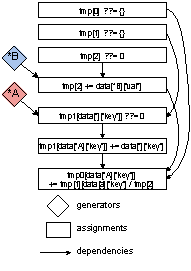
\includegraphics{images/intro_ir.pdf}
% \end{minipage}
% \begin{minipage}{0.62\textwidth}
% \begin{lstlisting}[style=JavaScript,columns=flexible]
% let tmp = {}
% tmp[0] ??= {}
% tmp[1] ??= {}                   
% tmp[2] ??= 0                        
% // sub-query de-correlated (loop hoisted)
% (*@\highlight[highlightblue]{for (let b in data)}@*) {
%   tmp[2] += data[b]["val"]      // computes full aggregate
% }
% (*@\highlight[highlightred]{for (let a in data)}@*) {
%   tmp[1][data[a]["key"]] ??= 0
%   tmp[1][data[a]["key"]] +=
%             data[a]["key"]      // computes partial aggregate
%   tmp[0][data[a]["key"]] = 
%             tmp[1][data[a]["key"]] / tmp[2] // proportion
% }
% \end{lstlisting}
% \end{minipage}
% \caption{
% On the left is the generated IR for the query in (a), comprising generators
% (diamonds) representing iterators and assignments (rectangles) corresponding
% to computations.
% On the right is the JS code generated from this IR.
% Notably, the `inner query' is hoisted in the final
% generated code.
% }\label{fig:ir_code}
% \end{subfigure}

% \caption{
% The end-to-end workflow of \lang{}, starting with the query (a),
% followed by the construction of the IR on the left side of (b), and the
% final generated code on the right side of (b).
% \todo{have a simpler example here.}
% \todo{src | IR | generated code}
% }\label{fig:intro}
% \end{figure}


\begin{figure}[t!]
\begin{subfigure}{\textwidth}
\begin{minipage}{0.25\textwidth}
\begin{lstlisting}[style=JavaScript, columns=flexible]
// input dataset
let data = [
  {key: "A", val: 10},
  {key: "B", val: 15},
  {key: "A", val: 25}
]
// query (result: 50)
sum('data.*.val')
\end{lstlisting}
\end{minipage}
\begin{minipage}{0.21\textwidth}
\centering
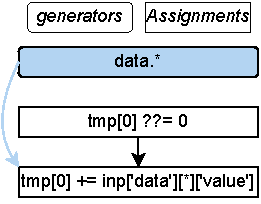
\includegraphics[width=0.9\textwidth]{images/intro_q1_ir.pdf}
\end{minipage}
\begin{minipage}{0.54\textwidth}
\begin{lstlisting}[style=JavaScript, columns=flexible, numbers=left, xleftmargin=2pt]
let tmp = {}
tmp[0] ??= 0
(*@\highlight[highlightblue]{for (let star in data) }@*) {
    tmp[0] += data[star]['val']
}
return tmp[0]
\end{lstlisting}
\end{minipage}
\caption{A query computing the sum of all values}\label{fig:intro_q1}
\end{subfigure}

\begin{subfigure}{\textwidth}
\begin{minipage}{0.25\textwidth}
\begin{lstlisting}[style=JavaScript, columns=flexible]
// query
{
 total: sum('data.*.val'),
 'data.*.key': sum('data.*.val')
}
/* result:
 { total: 50, 
   'A': 35,
   'B': 15 } */
\end{lstlisting}
\end{minipage}
\begin{minipage}{0.21\textwidth}
\centering
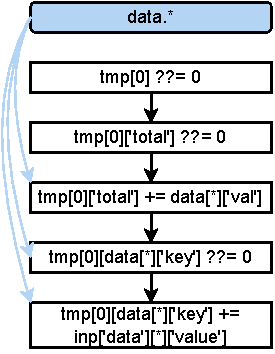
\includegraphics[width=0.9\textwidth]{images/intro_q2_ir.pdf}
\end{minipage}
\begin{minipage}{0.54\textwidth}
\begin{lstlisting}[style=JavaScript, columns=flexible, numbers=left, xleftmargin=2pt]
let tmp = {}
tmp[0] ??= {}
tmp[0]['total'] ??= 0
(*@\highlight[highlightblue]{for (let star in data) }@*) {
  tmp[0]['total'] += data[star]['val']
  tmp[0][data[star]['key']] ??= 0
  tmp[0][data[star]['key']] += data[star]['value']
}
return tmp[0]
\end{lstlisting}
\end{minipage}
\caption{A query computing sum of all values
(\inline{total}) and sum per each key}\label{fig:intro_q2}
\end{subfigure}

\begin{subfigure}{\textwidth}
\begin{minipage}{0.25\textwidth}
\begin{lstlisting}[style=JavaScript, columns=flexible]
// query
{
  'data.*A.key': 
   div(sum('data.*A.val'),
       sum('data.*B.val')) 
}
// result:
// {'A': 0.7, 'B': 0.3}
\end{lstlisting}
\end{minipage}
\begin{minipage}{0.21\textwidth}
\centering
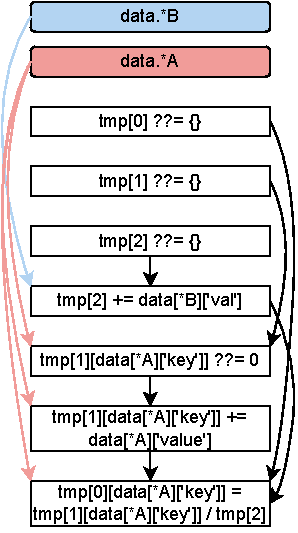
\includegraphics[width=0.9\textwidth]{images/intro_q3_ir.pdf}
\end{minipage}
\begin{minipage}{0.54\textwidth}
\begin{lstlisting}[style=JavaScript, columns=flexible, numbers=left, xleftmargin=2pt]
let tmp = {}
tmp[1] ??= {}
tmp[2] ??= 0
(*@\highlight[highlightblue]{for (let starB in data)}@*) {  // loop hoisted!
  tmp[2] += data[starB]['val']
}
tmp[0] ??= {}
(*@\highlight[highlightred]{for (let starA in data)}@*) {
  tmp[1][data[starA]['key']] ??= 0;
  tmp[1][data[starA]['key']] += data[starA]['val']
  tmp[0][data[starA]['key']] = tmp[1][data[starA]['key']] / tmp[2] (*@\label{line:deps}@*)
}
return tmp[0]
\end{lstlisting}
\end{minipage}
\caption{A query computing key-specific relative aggregate proportions}\label{fig:intro_q3}
\end{subfigure}
\caption{
The end-to-end workflow of \lang{} for three queries, starting with the query (left),
followed by the construction of the IR (mid), and the final generated code (right).
}\label{fig:intro}
\end{figure}

In \Cref{fig:intro}, we show a glimpse of how our query language works end-to-end.
Note that our current implementation is done in JavaScript (JS) and we generate JS
code for given input queries.
As shown in \Cref{fig:intro_q1}, the dataset for these examples consists of a collection
of objects, each featuring a \inline{key} and a \inline{val}.
The query in \Cref{fig:intro_q1} is a simple query that computes the sum of all
\inline{val} values.
Here, the \inline{*} symbol serves as an iterator, facilitating iteration through
the \inline{val} values, while the reducer \inline{sum} calculates the sum of
these iterated values.

In the middle section of the figure, we show the IR constructed from this query.
\lang{}'s IR consists of two main types of operators.
First, it has generators (represented as \emph{rounded} rectangles), which represents iterators
that iterates through a list of items (ultimately translated into loops within
the generated code).
In our example, \inline{data.*} is a generator, iterating values from the data object.
Second, the IR has assignments (represented as rectangles), comprising the
computations required for executing the query.
In the case of our first query, the initialization logic \inline{tmp[0] ??= 0} and
the subsequent sum computation \inline{tmp[0] += ...} are assignments.

Notably, the IR operates without the need for explicit control flow constructs.
Instead, the program's structure is implicitly inferred through dependencies.
For our example query, the update assignment \inline{tmp[0] += ...} has dependencies to
both the initializer (because have to initialize first) and the generator
(because its operand is the iterated value).
Additionally, it is worth noting that computations are performed on temporary
state variables (\inline{tmp[0]} in the first example).
This approach, utilizing intermediate temporaries, draws inspiration from works
such as RPAI~\cite{rpai} and DBToaster~\cite{dbtoaster_vldb}.
These systems utilize state variables (or maps) to maintain values for
various sub-queries of the main query, which are then leveraged to compute the
final result.
Finally, the IR is translated into JS code, taking dependencies into account to
extract the program structure and performing optimizations as part of this
transformation process.

\Cref{fig:intro_q2} and \Cref{fig:intro_q3} illustrate two additional queries executed on
the same dataset.
Specifically, in \Cref{fig:intro_q2}, we compute both the total sum of all values
(similar to the query in \Cref{fig:intro_q1}) and the sum of values per key, effectively
a group-by sum operation.
A key characteristic of \lang{} lies in the contextual interpretation of expressions
such as \inline{sum(data.*.val)}.
That is, the semantics of this expression differs depending on its context.
For instance, when it is nested within \inline{data.*.key},
it signifies a group-by sum operation.
Conversely, if it is not nested within an iterator (i.e., \inline{*}),
it calculates the aggregate over the entire set of values.
This distinction is exemplified in the query presented in \Cref{fig:intro_q3}.
Here, \inline{sum(data.*A.val)} is nested within \inline{data.*A.key}, signifying a
group-by aggregate operation.
Conversely, \inline{sum(data.*B.val)} computes a total aggregate, as it is not nested
within a \inline{*B} iterator.

Additionally, \Cref{fig:intro_q3} also demonstrates an optimization that occurs at the IR level.
Specifically, even though the \inline{sum(data.*B.val)} appears as a nested sub-query
in the original query, the \lang{} backend can determine that the generated
\inline{*B} can be hoisted out as a separate loop by analyzing the IR dependencies.
This is essentially similar to sub-query hoisting that happens at logical plan level
in other traditional query optimizers.

These examples provide a broad overview of \lang{}'s functionalities and its
syntax structure.
In the subsequent sections of this paper, we will delve deeper into the syntax and capabilities
of \lang{} and discuss the process of IR construction and code generation.
Moreover, the previous example queries exemplified \lang{}'s capability to
express analytical queries on JSON objects.
However, the versatility of \lang{} extends beyond this, encompassing an even broader
spectrum of use cases. 
For example, this includes its ability to 
express tensor computations in a style similar to
Einstein notation as we discuss in \Cref{subsec:tensor}.

Our specific contributions are as follows.

\begin{itemize}
    \item We present the syntax of our query language and demonstrate how to express common
          data manipulation operators like, selections, group-bys, joins, user-defined functions (UDFs),
          and so on.
          Moreover, we show how \lang{} can be used to express complex tensor computations in a declarative
          manner similar to Einsum notation (\Cref{sec:query_language}).
    \item We show how the queries are lowered into an IR that contains loop-free and branch-free code
          with dependencies implicitly representing the program structure.
          Then, we demonstrate how this IR can be used to generate code for a given query by constructing
          the program structure from dependencies.
          Moreover, we show how traditional compiler optimizations like lambda lifting translates to query
          optimizations like sub-query de-correlation (\Cref{sec:ir_codegen}).
    % \item We demonstrate the capabilities of our overall query language by taking a relatively simple example
    %       program that uses most of the features we have presented in previous sections (\Cref{sec:case_study}).
    \item We compare the performance of \lang{} on several practical JSON analytics workloads to demonstrate the
          effectiveness of our code generation approach (\Cref{sec:experiments}).
\end{itemize}

We discuss related work in \Cref{sec:related_work}, followed by conclusions and potential future research directions
in \Cref{sec:conclusions}.


\section{The Query Language}~\label{sec:query_language}

In the previous section, we saw \lang{} in action for a set of relatively simple queries.
In this section, we will introduce the syntax of the \lang{}, illustrating how it facilitates
the expression of common data manipulation operations like selections, aggregates,
group-bys, and so on.
To enhance comprehension, we will employ a running illustrative example dataset, as
depicted below.
Specifically, we have a dataset containing population of several major cities,
along with the respective country.
Our chosen dataset is deliberately kept relatively straightforward, devoid of
intricate nested structures.
However, it is worth noting that \lang{} has the capacity to seamlessly query
deeply nested JSON data without any problem in the same way.


\begin{lstlisting}[style=JavaScript]
let data = [
    {country: "Japan", city: "Tokyo",     population: 14},
    {country: "China", city: "Beijing",   population: 22},
    {country: "France",city: "Paris",     population: 3},
    {country: "UK",    city: "London",    population: 9},
    {country: "Japan", city: "Osaka",     population: 3},
    {country: "UK",    city: "Birmingham",population: 2}
]
\end{lstlisting}

\subsection{Basics}
First we will look at how to perform several basic query operations on the
aforementioned dataset.
For instance, if we want to select a particular key of the dataset at a given
index, we can use the following syntax.

\begin{lstlisting}[style=JavaScript]
'data.0.country'              // result: Japan
{first : 'data.0.country'}    // result: {first: Japan}
\end{lstlisting}

Several key attributes of \lang{} can be observed from the aforementioned examples.
In the given illustration, the reference \inline{data} refers to
the dataset object, enabling simple indexing into the array of data through integer
indices.
Furthermore, the selection of specific keys is facilitated by specifying the desired
key names (e.g., \inline{.country}).
Notably, \lang{} offers the convenience of the familiar JS-like syntax for constructing
structured output from extracted values, as exemplified in the second instance.

While this form of explicit indexing into the array can be useful for several
use cases, generally, queries involve some form of iterating over the dataset.
\lang{} offers this capability through the \inline{*} operator,
serving as an implicit iteration operator.
Later in our discussion, we will delve into how this operator empowers fine-grained
iterations, utilizing multiple iterators
(e.g., \inline{*A}, \inline{*B}, etc.).
For now, our focus centers on relatively simple queries.
Below, we present three example queries that leverage iterators and compute
aggregates over the iterated values.

\begin{lstlisting}[style=JavaScript, columns=flexible]
['data.*.city']             // result: [Tokyo, Beijing, ..., Birmingham]
sum('data.*.population')    // result: 53
max('data.*.population')    // result: 22
\end{lstlisting}

The queries presented above are self-explanatory in nature.
In the first example, we illustrate a scenario where an array can be constructed
from the values obtained through iteration, employing the \inline{[...]} syntax.
Alternatively, users can compute aggregates over the iterated values using the
relevant aggregate functions, such as \inline{sum}, \inline{max}, and so forth.
As discussed previously, this queries can be used as parts of object
construction logic and combined flexibly as shown below.

\begin{lstlisting}[style=JavaScript, columns=flexible, numbers=none]
{ total: sum('data.*.population'), maximum: max('data.*.population') }
// result: {total: 53, max: 22}
\end{lstlisting}

% \begin{minipage}{0.5\textwidth}
% \begin{lstlisting}[style=JavaScript, columns=flexible, numbers=none]
% { 
%     total: sum(data.*.population),
%     maximum: max(data.*.population) 
% }
% \end{lstlisting}
% \end{minipage}

% \begin{minipage}{0.5\textwidth}
% \begin{lstlisting}[style=JSComment, columns=flexible, numbers=none]
% result: 
% {
%     total: 53,
%     max: 22
% }
% \end{lstlisting}
% \end{minipage}


\subsection{Group By}\label{subsec:groupby}
Up to this point, we have explored fundamental query operations, including indexing,
iteration, and aggregate computation.
Another vital query operator, especially relevant to JSON-style objects,
is the group-by query.
\lang{} offers an intuitive means of implicitly expressing group-bys.
The following query exemplifies this, grouping records based on the
\inline{country} attribute and subsequently calculating the total population
for each group:

\begin{lstlisting}[style=JavaScript, columns=flexible, numbers=none]
{ 'data.*.country': sum('data.*.population') }
// result: {Japan: 17, China: 22, France: 3, UK: 11}
// SQL: SELECT country, SUM(population) FROM data GROUP BY country;
\end{lstlisting}

In the above syntax, specifying \inline{data.*.country} as the key implies
that any iteration carried out within this key utilizing the same
iterator (\inline{*}) is performed for records with each unique value of \inline{country}
separately.

The next example shown below demonstrates the versatility of \lang{} group-by queries, showcasing
aggregations at different levels.
Moreover, it shows the composability of \lang{} queries.
This query computes the total population of all records, breaks it down by country,
and subsequently computes the population proportion of each city with respect to its
corresponding country:

\begin{lstlisting}[style=JavaScript, columns=flexible, numbers=none]
let countryPop = {'data.*A.country': sum('data.*A.population')}// country -> population
let query = { 
    total: sum('data.*.population'),                                  // total population
    'data.*.country':
    {   total: get(countryPop, 'data.*.country')                      // population per country
        'data.*.city': div(sum('data.*.population'),                  // population proportion
                            get(countryPop, 'data.*.country'))}       // (per each city)
}
// result: {total: 53. Japan: {total: 17, Tokyo: 0.82, Osaka: 0.18}, ...}
\end{lstlisting}

Specifically, the \inline{countryPop} is a separate query that determines the total
population for each country.
This query is subsequently used within the main \inline{query} to access the
total population for each country where required.
As we saw in \Cref{fig:intro_q3}, \lang{}'s backend optimizes the
query by hoisting the independent \inline{*A} iterator outside and performing
a lookup on the reified \inline{countryPop} instead of computing the
corresponding aggregate inside a nested loop.

\subsection{Join}
Joins are another fundamental operator in data querying.
To illustrate how joins work in \lang{}, consider the following
new dataset named \inline{other}, which includes information about the
\inline{region} to which each country belongs:

\begin{lstlisting}[style=JavaScript, columns=flexible]
let other = [
    {country: "Japan", region: "Asia"},
    {country: "China", region: "Asia"},
    {country: "France",region: "Europe"},
    {country: "UK",    region: "Europe"},
]
\end{lstlisting}

Now, let's consider a scenario where we aim to compute aggregate population
values based on regions.
To achieve this, we must perform a join operation between our original
\inline{data} object and this new \inline{other} object to acquire the
corresponding region for each country.
The following \lang{} query demonstrates how such an operation can be
expressed:

\begin{lstlisting}[style=JavaScript, columns=flexible]
let countryToRegion = {
    'other.*O.country': 'other.*O.region'
}
let query = {
    "-": keyval(get(countryToRegion, 'data.*.country'), {
        total: sum('data.*.population')
        'data.*.country' : sum('data.*.population')
    }),
}
// result: {Asia: {total: 39, Japan: 17, China: 22}, Europe: {total: 14, France: 3, UK: 11}}
\end{lstlisting}

As with the example in \Cref{subsec:groupby}, we employ a distinct query
(\inline{countryToRegion}) to map countries to regions.
The \inline{keyval(<key>, <value>)} construct is utilized to specify the mapped region
as the key.
This query conducts a group-by based on the \inline{region} attribute initially,
followed by another group-by based on \inline{country}, ultimately calculating the
desired aggregates.

% \todo{perhaps discuss this in future work}
% \subsection{Conditionals}
% \todo{
%     discuss about expressing filters. Duality with lambdas + if.
% }
% One approach to handle conditionals is to provide 

% \begin{lstlisting}[style=JavaScript, columns=flexible]
% data2Map = {"data2.*.key": sum("data2.*.value")}
% query = {"data.*.key": get(data2Map, "data2.*.value")}

% // RPAI-style maps
% // select sum(r.A*r.B) from R r where 
% // 0.5*(select sum(r1.B) from R r1) == (select sum(r2.B) from R r2 where r2.A = r.A)
% lhsSum = sum(r.*p.B)
% rhsSum = { "r.*q.A": sum("r.*q.B")} // A --> rhsSum

% // TODO: how to express this declaratively?
% ansMap = { ???: sum(times("r.*q.A", "r.*q.B")) } // rhsSum --> sum(A*B)
% // need a way to encode shift of aggregates! 
% query = get(ansMap, lhsSum)
% \end{lstlisting}

\subsection{User-defined Functions}
\lang{} allows using user-defined functions (UDFs) written in JS seamlessly with the
queries.
Consider a simple query where we want to obtain the percentage population per each
country from our dataset.

\begin{lstlisting}[style=JavaScript, columns=flexible]
let udf = {
    formatPercent: v => (v*100).toFixed(2) + "%" // computes the percentage 
}
let query = {
    'data.*.country':
        apply(udf.formatPercent, div(sum('data.*.population'), sum('data.*A.population')))
}
// result: {Japan: 32.05%, China: 41.50%, France: 5.66%, UK: 20.75%}
\end{lstlisting}

We have defined the \inline{formatPercent} that given a proportion value (float),
computes the percentage and adds a \% sign at the end.
We can then use \inline{apply} in the query to call this UDF to convert the
proportions to percentages.


\subsection{Arrays}
We have encountered aggregates such as \inline{max}, \inline{min}, and \inline{sum}
thus far.
However, there can be scenarios where we require an aggregate that collects values
into an array.
For this, we provide the \inline{array} construct, also represented in \inline{[]} syntax.

\begin{lstlisting}[style=JavaScript, columns=flexible]
array('data.*.country')                                   // [Japan, China, France, ...]
[{city: 'data.*.city'}]                                   // [{city: Tokyo}, {city: Beijing}, ...]
[{country: 'data.*.country'}, {city: 'data.*.city'}]// [{country: Japan}, {city: Tokyo}, ...]
[{country: 'data.*.country', city: 'data.*.city'}]        // [{country: Japan, city: Tokyo}, ...]
\end{lstlisting}

In the examples provided above, we show a set of simple queries that aggregate values
into arrays.
Each query is self-explanatory, with the expected result displayed on the right.
Importantly, similar to other types of \lang{} operations, this array accumulation
seamlessly integrates with other query constructs.

\subsection{Fluent API}
Sometimes, the JSON-style query interface can be cumbersome,
especially when dealing with deeply nested objects.
To address this issue, \lang{} offers a higher-level API that employs
metaprogramming to compose queries more easily.
This `fluent' API provides a pipeline-oriented interface that
simplifies complex queries.

To illustrate the advantages of this interface, let us consider a
simple task borrowed from Advent of Code 2022~\cite{adventofcode22}.
The task involves processing a sequence of values partitioned into chunks,
each containing multiple values.
The objective is to calculate the sum of values for each chunk and
subsequently identify the maximum sum among those computed.
To begin, let's examine how the \lang{} query appears when utilizing
the familiar JSON-style API for data parsing and computation.


\begin{lstlisting}[style=JavaScript, columns=flexible]
let input = '100,200,300|400|500,600|700,800,900|1000' // sample input
// some UDFs for parsing the data
let udf = {
    'splitPipe' : x => x.split('|'),
    'splitComma': x => x.split(','),
    'toNum'      : x => Number(x)
}
\end{lstlisting}

First, we define several user-defined functions (UDFs) to assist with data parsing.
The role of each UDF is simple and self-explanatory.
Shown below is the \lang{} query responsible for executing the required
computation, with comments provided alongside to elucidate each section
of the query (numbered for clarity):

\begin{lstlisting}[style=JavaScript, columns=flexible, numbers=left]
let query = max(get({                      // 5. find maximum among group sums
    '*chunk': sum(                         // 4. group-by chunk and compute sum
        apply('udf.toNum',                 // 3. convert each string number to a number object
            get(apply('udf.splitComma',    // 2. split by comma to get numbers of each chunk
                get(apply('udf.splitPipe', '.input'), '*chunk')), // 1. split into chunks
            '*line')))
    },'*'))
\end{lstlisting}

\inline{apply()} is used to apply UDFs to arguments.
\inline{get()}, when used with an unbounded generator symbol (e.g., \inline{*chunk}), binds the
iterator to the object in the first argument.
For example, in Line 5, \inline{get(..., '*chunk')} binds the iterator
\inline{*chunk} to the result of splitting the output by the pipe symbol (\inline{|}).
While this approach works as intended and yields the correct results, it can certainly be
a bit too cumbersome to write the query in this deeply nested manner.
In such cases, \lang{}'s `fluent' interface offers an alternative to express
this query concisely as shown below.


\begin{lstlisting}[style=JavaScript, columns=flexible]
let query =
    pipe('.input')
    .map('udf.splitPipe').get('*chunk')      // 1. split into chunks (and bind to *chunk)
    .map('udf.splitComma').get('*line')      // 2. split by comma to get numbers of each chunk
    .map('udf.toNum')                        // 3. convert each string number to a number object
    .sum().group('*chunk').get('*')          // 4. group-by chunk and compute sum
    .max()                                   // 5. find maximum among group sums
\end{lstlisting}

In this new version, you can observe that this high-level interface provides a
much cleaner and more concise way to express the same query. 
This high-level fluent API essentially functions as a metaprogramming layer
that generates an equivalent query to the one we saw previously.
The \inline{pipe()} function creates a \inline{Pipe} object equipped with
APIs such as \inline{sum}, \inline{max}, and so on, all of which return a
\inline{Pipe}.
The \inline{map()} function, similar to \inline{apply()} mentioned earlier,
is employed to apply a UDF, and \inline{group()} is used to perform a group-by.


% \subsection{GUI Components}
% Basic building blocks -- table definition, and generic display, svg, etc. 

\begin{figure}[t]
\begin{minipage}{0.5\textwidth}
\begin{lstlisting}[style=JavaScript, columns=flexible, numbers=left]
// some simple input tensors
let A = [[1, 2], [3, 4]]
let B = [[1, 2, 3], [4, 5, 6]]

// tensor transpose (ij->ji)
{'*j': {'*i': 'B.*i.*j'}}
// result: {0: {0: 1, 1: 4}, 1: {0: 2, 1: 5},
//           2: {0: 3, 1: 6}}

// sum of all elements (ij->)
sum('B.*i.*j')
// result: 21

// column sum (ij->j)
{'*j': sum('B.*i.*j')}
// result: {0: 5, 1: 7, 2: 9}

// row sum (ij->i)
{'*i': sum('B.*i.*j')}
// result: {0: 6, 1: 15}

// matrix multiplication (ik,kj->ij)(*@\label{code:matmulquery}@*)
{'*i': {'*j': sum(
    times('A.*i.*k', 'B.*k.*j')) }}
// result: {0: {0: 9, 1: 12, 2: 15},
//           1: {0: 19, 1: 26, 2: 33}}
\end{lstlisting}
\end{minipage}
\begin{minipage}{0.5\textwidth}
\begin{lstlisting}[style=JavaScript, columns=flexible, numbers=left, firstnumber=last]
// diagonal (ii -> i)
{'*i': 'A.*i.*i'}
// result: {0: 1, 1: 4}

// Hadamard product (ij,ij->ij)
{'*i': {'*j': times('A.*i.*j', 'B.*i.*j') }}
// result: {0: {0: 1, 1: 4}, 1: {0: 9, 1: 16}}

// dot product (vector-vector) (i,i->)
sum(times('vecA.*i', 'vecB.*i'))

// batched matmul (bik,bkj->bij)
// T1 and T2 are tensors
// T1: BxIxK, T2:BxKxJ (B is batch-dim)
{'*b': {'*i': {'*j': sum(
    times('T1.*b.*i.*k', 'T2.*b.*k.*j')) }}}

// general tensor contraction
// e.g., pqrs,tuqvr->pstuv
{'*p':{'*s':{'*t':{'*u':{'*v':sum(
    times('T1.*p.*q.*r.*s', 'T2.*t.*u.*q.*v.*r')) }}}}}

// bi-linear transformation (ik,jkl,il->ij)
{'*i': {'j': sum(times(
    'T1.*i.*k', 'T2.*j.*k.*l', 'T3.*i.*l'))} }
\end{lstlisting}
\end{minipage}
\caption{
Shows how \lang{} is used to express tensor computations declaratively:
from basic tensor operations (e.g., summation, row, and column sums) to relatively complex expressions
(e.g., general tensor contractions, three-tensor bilinear transformations), similar
to Einsum notation.
We can observe that \lang{} queries
mirror the corresponding Einsum equations (shown in parenthesis).
Examples are taken from~\cite{einsumblog}.
}\label{fig:tensors}
\end{figure}


\subsection{Tensor Expressions}\label{subsec:tensor}
In the preceding subsections, we have explored how \lang{} enables expressive
manipulation of JSON-like data, demonstrating its utility in various contexts.
However, \lang{}'s versatility extends beyond typical data workloads.
Notably, \lang{} provides an elegant framework for expressing tensor computations,
drawing inspiration from the Einstein summation (Einsum) notation frequently
employed in tensor frameworks.

The Einsum notation offers a concise means of articulating tensor computations.
For instance, the expression $ik,kj \rightarrow ij$ specifies a tensor operation
that takes two two-dimensional tensors (say $A$ and $B$), and yields a third
tensor (say $C$), as the result, computed as $C_{ij} = \sum_k A_{ik} \times B_{kj}$.
Likewise, complex tensor computations involving multiple n-dimensional tensors can
be specified using such declarative expressions.

\lang{} provides the means to express tensor computations in a declarative fashion,
as illustrated in \Cref{fig:tensors}.
The structure of a \lang{} query closely mirrors the corresponding Einsum equation.
Notably, the keys (indices) following the `$\rightarrow$' symbol transition into keys
within the query, while the equation's body simply becomes the corresponding tensors
with their respective indices (i.e., \inline{*i}, \inline{*j}, and so on).
For instance, consider matrix multiplication expressed in Einsum notation as
$ik,kj \rightarrow ij$.
This equation simply translates into a \lang{} query (\Cref{fig:tensors}, Line~\ref{code:matmulquery}) featuring \inline{*i} and
\inline{*j} as query keys. The body of the query comprises the two matrices, accessed as
\inline{A.*i.*k} corresponding to $ik$ and \inline{B.*k.*j} corresponding to $kj$.

\Cref{fig:tensors} shows how \lang{} can be leveraged to express a variety of
tensor expressions, ranging from simple queries like sums or sums along
dimensions (e.g., rows or columns for matrices) to more complex expressions
such as general tensor contractions for n-ary tensors and expressions like
bilinear transformations that involve three tensors. 
To mirror Einsum-style reductions, we employ \inline{sum(times(...))}.
However, it is important to note that users have the freedom to choose
any type of reductions beyond just $\sum$ and $\times$, allowing more flexibility.

You may have observed that the iterators (e.g., \inline{*}, \inline{*i}, etc.) in these
examples differ somewhat from what we encountered previously.
Specifically, in prior cases, we explicitly specified the data source from which we iterate,
as seen in constructs like \inline{data.*A}.
However, here, we only specify the iterator as the key, and \lang{}'s backend
automatically determines the appropriate data source by examining the query body.
For instance, when we have a query like \inline{\{*i: sum(times(A.*i, B.*i))\}}, the
backend selects either \inline{A} or \inline{B} as the data source for iteration.
Subsequently, the generated code ensures that the iterated values exist in
both \inline{A} and \inline{B}.
For readers familiar with languages like Datalog, this concept essentially
parallels unification.

% Another key benefit of \lang{} is that these queries, for the most part are agnostic
% to the underlying data structure.
% For instance, one could use a JSON to represent a sparse tensor in a format similar to
% coordinate list (COO) format (e.g., this is the format used in \inline{SparseTensor}
% in TensorFlow) and use the same query to perform a matrix multiplication.
% \begin{lstlisting}[style=JavaScript, columns=flexible]
% let sparseA = [{row: 0, col: 1, val: 1}, {row: 1, col: 0, val: 2}] // [[0, 1], [2, 0]]
% let sparseB = [{row: 0, col: 0, val: 2}, {row: 0, col: 1, val: 1}] // [[2, 1], [0, 0]]
% // query TODO!
% {'*i': {'*j': sum(times('sparseA.*i))}}
% \end{lstlisting}

These queries also go through the same compilation steps as we saw in \Cref{fig:intro}.
Specifically, these queries get translated into a loop-free, branch-free IR that contains the
operators corresponding to the tensor expressions that then get translated into
optimized JS code.

\section{IR and Code Generation}~\label{sec:ir_codegen}

Up to this point, we have provided an introduction to the syntax of
\lang{} and explored its versatility across various domains.
In \Cref{fig:intro}, we gained a preliminary understanding
of how \lang{} queries are transformed into an IR, which subsequently serves
as the basis for generating optimized code.
In this section, we will delve into a detailed discussion of the IR structure
and the code generation process.

\subsection{IR Structure}
As discussed in \Cref{sec:intro}, the IR structure of \lang{} consists of two
primary types of instructions: \emph{generators} and \emph{assignments}.
Generators correspond to iterators responsible for enumerating input or intermediate
nested objects, and these generators are transformed into loops in the generated code.
Assignments, on the other hand, encompass any form of computation that updates or
initializes an intermediate or output state.

\lang{} queries inherently exhibit nested iterating structures that could be simply
translated into a series of nested loop structures in the generated code.
However, performing this transformation naively and enforcing the `program structure'
implied by the user query would lead to missed optimization opportunities like
hoisting computations and loops that are independent of outer loops,
common sub-query/expression elimination, and more.
Therefore, rather than naively transforming queries and directly imposing the program
structure, we extract a set of generators, iterators, and their dependencies during
IR construction.
While the IR does not explicitly capture the program structure, the optimal program
structure can be derived from an analysis of these dependencies.

The dependency structure is relatively straightforward.
As demonstrated in the generated code snippet in \Cref{fig:intro}, we utilize objects such
as \inline{tmp[0]}, \inline{tmp[1]}, and so on, to maintain intermediate results required
for computing the final query result.
Assignment operators have these temporaries as operands, creating data dependencies in the
process.
Generators can also iterate values from these temporaries, and in such cases, we introduce
similar dependencies for the generators.
Similarly, when a generator symbol is used in an assignment or another generator, a
dependency is added.
To illustrate how dependencies are created, consider the following assignment instruction
extracted from Line~\ref{line:deps} in \Cref{fig:intro_q3}:

\begin{lstlisting}[style=JavaScript, columns=flexible, numbers=left, firstnumber=11]
tmp[0][data[starA]['key']] = tmp[1][data[starA]['key']] / tmp[2]
\end{lstlisting}

This instruction relies on \inline{tmp[0]}, \inline{tmp[1]}, and \inline{tmp[2]} as operands.
As a result, this instruction is associated with the last (write) operations of all three
temporaries as dependencies, as depicted in the IR visualization presented in \Cref{fig:intro_q3}.
Furthermore, since it employs the \inline{*A} iterator, it also exhibits a dependency on the
corresponding generator.

% In our current implementation, we track dependencies at the granularity of temporaries like
% \inline{tmp[0]}, \inline{tmp[1]}, etc.
% Specifically, we assign a write rank for each assignment and enforce the strict ordering of
% write ranks during code generation.
% But we can do this in a granular way --> essentially treating each writeRank as an SSA variable
% and track dependencies at that level
% \todo{should we mention this?}

\subsection{Constructing the IR}
\todo{mention How the \lang{} queries are transformed to the IR.
Discuss path, how and when new temps are created, etc.}

\subsection{Code Generation}
Once the IR is constructed for a query, next step is to generate the final code
taking into account the instruction dependencies.
This phase involves the crucial task of determining the program structure from
the dependencies.
Specifically, it entails determining where to insert loops, how to nest loops
within one another, where to place assignment instructions, and so on. 
We will use the query from \Cref{fig:intro_q3} as a running example for this
section.

The first step in doing this involves identifying two key
components: \inline{tmpInsideLoop} and \inline{tmpAfterTmp}.
These variables serve the purpose of tracking which temporaries should be scheduled
inside particular loops and which temporaries should be scheduled after
certain other temporaries.
Shown below is an excerpt of the code doing that.
\inline{e.writeSym} refers to the left-hand side temp of assignments.
Shown on the right are \inline{tmpInsideLoop} (solid) and \inline{tmpAfterTmp} (dotted)
for query in \Cref{fig:intro_q3}.

\begin{minipage}{0.7\textwidth}
\begin{lstlisting}[style=JavaScript, columns=flexible]
// compute tmpInsideLoop and tmpAfterTmp
for (let e of assignmentStms) {
    for (let dep of e.deps) {
        // depends on a loop, it should be inside the loop
        if (isloop(dep)) tmpInsideLoop[e.writeSym][dep] = true
        // depends on a tmp, expression should be after that
        if (istmp(dep)) tmpAfterTmp[e.writeSym][dep] = true
}   }
\end{lstlisting}
\end{minipage}
\begin{minipage}{0.3\textwidth}
% \centering
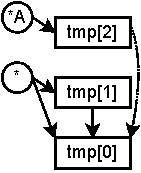
\includegraphics[width=0.5\textwidth]{images/q3_deps.pdf}
\end{minipage}

In the above code, we iterate through all the assignment statements and examine all
their dependencies.
If a statement depends on a loop, it means the corresponding temporary variable must
be scheduled inside the loop, thus updating the \inline{tmpInsideLoop} variable.
Furthermore, if an assignment depends on another temporary value, it means the
corresponding temporary variable must be scheduled after that, consequently updating
the \inline{tmpAfterTmp} variable.

The next step involves computing the \inline{tmpAfterLoop} based on the gathered information.
Specifically, if we determined that a temp \inline{t2} should be scheduled after
another temp \inline{t1} (i.e., \inline{tmpAfterTmp[t2][t1]}), which resides inside a loop \inline{l}
(with the condition that \inline{t2} itself is not within loop \inline{l}),
then this implies that \inline{t2} should be scheduled after the loop \inline{l}.
For instance, in our sample query, \inline{tmp[0]} should be scheduled after \inline{*A}.
Shown below is the code to implement this logic that populates the \inline{tmpAfterLoop}.

\begin{lstlisting}[style=JavaScript, columns=flexible]
// compute tmpAfterLoop
for (let t2 in tmpAfterTmp) {
    // gather loop 'prior' tmps are in
    for (let t1 in tmpAfterTmp[t2]) {
      for (let l in tmpInsideLoop[t1])
        tmpAfterLoop[t2][l] = true
    }
    // remove own loops
    for (let l in tmpInsideLoop[t2])
      delete tmpAfterLoop[t2][l]
}
\end{lstlisting}

Subsequently, as the final analysis step before code generation, we determine
\inline{loopAfterLoop} and \inline{loopInsideLoop}.
These essentially help identify how the loops should be scheduled.
In particular, if we ascertain that a given temp \inline{t} should be scheduled
inside both loops \inline{l1} and \inline{l2}, it implies that \inline{l1} and
\inline{l2} should belong to the same loop nest.
Conversely, if we determined that for a particular temp \inline{t},
it resides within loop \inline{l2}, and we also know that \inline{t} should be
scheduled after another loop \inline{l1}, then this indicates that the loop \inline{l2}
should be scheduled after \inline{l1} (provided they are not part of the same loop nest).
The corresponding code for both of these analyses is presented below.

\hspace{-18pt}
\begin{minipage}{0.5\textwidth}
\begin{lstlisting}[style=JavaScript, columns=flexible]
// compute loopInsideLoop
for (let t in tmpInsideLoop) {
    for (let l2 in tmpInsideLoop[t]) {
        for (let l1 in tmpInsideLoop[t]) {
            loopInsideLoop[l2][l1] = true
            loopInsideLoop[l1][l2] = true
        }
    }
}
\end{lstlisting}
\end{minipage}%
\begin{minipage}{0.5\textwidth}
\begin{lstlisting}[style=JavaScript, columns=flexible]
// compute loopAfterLoop
for (let t in tmpAfterLoop) {
    for (let l2 in tmpInsideLoop[t]) {
        for (let l1 in tmpAfterLoop[t]) {
            if (!loopInsideLoop[l2][l1])
                loopAfterLoop[l2][l1] = true
        }
    }
}
\end{lstlisting}
\end{minipage}

Once the analysis steps are completed, we proceed with the code
generation process.
Our approach to code generation draws inspiration from the IR scheduling
algorithm utilized in Lightweight Modular Staging (LMS).
In particular, we schedule generators and assignments in an
`outside-in' fashion, commencing with the outer loops before
progressing to the inner ones.


The core driver of the code emission logic is encapsulated within
the \inline{emitConvergence} function. 
This function relies on two helper functions: \inline{emitGenerators}
and \inline{emitAssignments}.
The former is responsible for emitting loop structures, while the
latter deals with the generation of assignment instructions.
These functions are invoked repeatedly until all generators and
assignments are fully emitted.
We present an excerpt from the \inline{emitGenerators} function below:

\begin{lstlisting}[style=JavaScript, columns=flexible]
function emitGenerators() {
    let (available, remaining) = getAvailable(generators) // identify current scope loops
    generators = remaining              // remaining generators that are not available yet
    for (let g of available) {
        emitLoopHeader(g)
        emitConvergence()               // emit loop body (nested generators and assignments)
        emitLoopFooter()
    }
}
\end{lstlisting}

\inline{generators} here is as a global variable that keeps track of the
remaining generators that is yet to be scheduled.
The \inline{emitGenerators} function is responsible for orchestrating the
generation of loops corresponding to these generators.
It commences by identifying generators that become available in the
current scope, leveraging information such as \inline{loopAfterLoop},
\inline{tmpAfterTmp}, and others we saw before.
The \inline{getAvailable} function checks the dependencies of pending
generators and picks the ones where all dependencies are satisfied.
Consequently, this function schedules loops that are available at the
present scope and invokes \inline{emitConvergence} recursively to schedule
any inner loops and assignments that must be scheduled inside these loops.
\inline{emitAssignments} function follows a similar structure to that of
the \inline{emitGenerators}.
It schedules assignment instructions as soon as they become available in
the current context.

Since we did not have program control structures enforced from the front end,
this code scheduling mechanism freely schedules assignments and generators
in an optimal manner.
For instance, any generator that does not have dependencies to the `other query'
would be hoisted and scheduled as a separate query instead of repeating the
computation multiple times inside a nested loop.


\subsection{Implementation}
\todo{We implement this in <1000 lines of JavaScript, it can run in the browser, etc.}

% \section{Incremental}
% Incremental queries for JSONs, incremental tensor computations!



% \section{Example: Pivot Table}\label{sec:case_study}
% How to use group bys, partial aggregates, display, svg, etc.

\section{Experiments}\label{sec:experiments}
% We will have to variants: non-incremental and incremental.
% For incremental we can show the execution time per each `batch' of
% records (batch on x-axis).
\todo{simple query examples with synthetic key-value data (a simple aggr, group-By,
de-correlation, etc.). Compare against, JQ, JSONiq.}


\section{Related Work}\label{sec:related_work}
There are several query languages designed for working with semi-structured data like
JSON, each with its own focus and strengths.
JSONiq~\cite{jsoniq,jsoniq_paper} is a notable query language explicitly tailored for
JSON data, borrowing most of its syntax from XQuery~\cite{xquery} (e.g., FLWOR expressions).
Zorba~\cite{zobra} and RumbleDB~\cite{rumble_vldb} are examples of engines that support
JSONiq, with RumbleDB using Spark~\cite{spark} as a backend, leveraging the scalability
of Spark for execution.
AsterixDB, designed for semi-structured data, employs AQL~\cite{aql} and SQL++~\cite{sqlpp}
as its query languages.
GraphQL~\cite{graphql}, on the other hand, is widely used in web application development
for querying data from backend services.
Generally, resolvers for these queries should be manually implemented in the backend.
Some systems like Hasura~\cite{hasura} automate the generation of SQL queries from
GraphQL queries, simplifying query resolution.
Most of these languages are specifically targeted towards large-scale JSON analytics workloads.
While we take inspiration from these languages for the design of the language,
\lang{}, is designed to handle various forms of nested data,
including tensors, and it offers support for efficient code generation and optimizations
through its IR.

% We take inspiration from many other declarative programming languages.
% Specifically, this includes
% Logic programming, particularly, Datalog - choice and unification, einsum notation - for expressing tensor computations,
% implicit aggregation.
% Recent works like 

% Our generated code

\section{Conclusions and Future Work}\label{sec:conclusions}
Incrementality, Datalog-style recursive queries?, partial re-evaluation as
query changes (with minimal recomputation and index sharing)

\textbf{Incrementality} Although not discussed extensively in this paper, the idea
of using intermediate temporaries in the generated code is inspired by work in
incremental execution like DBToaster~\cite{dbtoaster_vldb} and RPAI~\cite{rpai}.
One of the immediate future works is to add support for incremental execution.

\textbf{Partial Re-evaluation}

\textbf{Missing Operators} sorting, arbitrary conditionals, etc.

\textbf{Cycles}

%
% ---- Bibliography ----
%
% BibTeX users should specify bibliography style 'splncs04'.
% References will then be sorted and formatted in the correct style.

\bibliographystyle{splncs04}
\bibliography{references}
\end{document}
